\documentclass{beamer}

\usefonttheme{professionalfonts}

\usetheme{Szeged}
\definecolor{beamer@jana}{rgb}{0.3, 0.6, 0.8}
\setbeamercolor{structure}{fg=beamer@jana}	
\usepackage{beamerthemeshadow}
\usepackage{url}
\usepackage[utf8]{inputenc}
\usepackage{graphicx}
\usepackage{color}
\usepackage{tikz}
\usepackage{caption}
\usepackage{subcaption}
\usepackage{dirtytalk}
\usepackage{amsthm}

\usepackage[]{algorithm2e}
\usepackage{algorithmicx}
\usepackage[Algorithm,ruled]{algorithm}
\usepackage{algorithm,algcompatible,amsmath}
\usepackage{mathtools}
\algnewcommand\DESCRIPTION{\item[\textbf{Opis:}]}%
\algnewcommand\INPUT{\item[\textbf{Ulaz:}]}%
\algnewcommand\OUTPUT{\item[\textbf{Izlaz:}]}%

\usepackage{fourier} 
\usepackage{array}
\usepackage{makecell}
\renewcommand\theadalign{cc}
\renewcommand\theadfont{\bfseries}
\renewcommand\theadgape{\Gape[2pt]}
\renewcommand\cellgape{\Gape[2pt]}

\usepackage{amsmath,bm}
\usepackage{adjustbox}

\setbeamertemplate{footline}{\hspace*{.5cm}\scriptsize{\hspace*{50pt} \hfill\hspace*{.5cm}}\\
\vspace{20pt}}

\usepackage[english,serbian]{babel}


\begin{document}
\title{\Large Metode za rešavanje problema simboličke regresije \\ \vspace{5pt} \scriptsize {master rad}\\ \vspace{2pt}\small{Jana Jovičić 1097/2019}\\ \vspace{2pt}\small{mentor: dr Aleksandar Kartelj}}
\institute {\tiny{Matematički fakultet\\Univerzitet u Beogradu}}
%\author{Jana Jovičić\\ \tiny 1097/2019}
\date{\tiny 26. septembar 2022.}

\setbeamertemplate{footline}
{
  \leavevmode
  \hbox{
  \begin{beamercolorbox}[wd=.49\paperwidth,ht=2.25ex,dp=1ex,center]{author in head/foot}
    \usebeamerfont{author in head/foot}{Jana Jovičić}
  \end{beamercolorbox}
  \begin{beamercolorbox}[wd=.49\paperwidth,ht=2.25ex,dp=1ex,center]{title in head/foot}
    \usebeamerfont{title in head/foot}{Master rad}
  \end{beamercolorbox}}
}


\begingroup
\setbeamertemplate{footline}{}
\begin{frame}
    \begin{tikzpicture}
        \node[anchor=north east, inner sep=2] (image) at (0,0)
        {
\includegraphics[width=1.8cm]{images/matf-light.png}};
        \node[anchor=north west, inner sep=2] (image) at (7,0)
        {
\includegraphics[width=1.3cm]{images/matf_logo.png}};
    \end{tikzpicture}
  \vspace{-0.53cm}
  \titlepage
\end{frame}
\endgroup

\setbeamertemplate{section in toc}[sections numbered]
\setbeamertemplate{subsection in toc}{\leavevmode\leftskip=3.2em\rlap{\hskip-2em\inserttocsectionnumber.\inserttocsubsectionnumber}\inserttocsubsection\par}
\setbeamerfont{subsection in toc}{size=\footnotesize}

\begin{frame}\frametitle{Sadržaj}\tableofcontents
\end{frame} 

\section{Uvod} 
\begin{frame} {Simbolička regresija (SR)} 
\begin{itemize}
\small
    \item Pronalazak matematičkog izraza u simboličkoj formi, koji dobro modeluje vezu između ciljne promenljive i nezavisnih promenljivih.
    \item Istovremeno uči i o strukturi modela i njegove parametre.
    %\item Prednost u odnosu na metode dubokog učenja -- lakša interpretabilnost.
    \item Problem kombinatorne optimizacije.
    \item Smatra se da je NP-težak problem. %, ali još nije formalno dokazano.
    %\item Najčešće se traže aproksimativna rešenja problema pomoću metaheurističkih metoda.
    \item Ako je dat skup podataka $(X_i, y_i)$, $i=1,...,m$, gde $X_i \in \mathbb{R}^{n}$ predstavlja $i$-ti skup atributa, a $y_i \in \mathbb{R}$ $i$-tu ciljnu promenljivu, cilj SR je pronalazak funkcije $f: \mathbb{R}^{n} \rightarrow \mathbb{R}$ koja najbolje odgovara skupu podataka, odnosno za koju važi $y_i \approx f(X_i), i=1,...,m$.
    \item Izraz se može predstaviti pomoću sintaksnog stabla.
\end{itemize}

\end{frame}


%%%%%%%%%%%%%%%%%%%%%%%%%%%%%%%%%%%%%%%%%%%%%%%%%%%%%

%\subsection{Evaluacija modela simboličke regresije}
\begin{frame}{Evaluacija modela simboličke regresije}
\begin{itemize}
\small
    \item Ranije - u terminima metaheuristike kojom je problem rešavan.
    \item Poslednjih godina - pomoću metrika kao što je koeficijent determinacije $R^2$ uz podelu skupa podataka na trening i test deo.
    \[ R^{2} = 1-\frac{MSE}{\operatorname{Var}(y)} \]
    %\item Uzima se u obzir i to da se jedna ista funkcija može izraziti pomoću više simbolički različitih zapisa.
    \item Smatra se da je ciljna funkcija $f$ ispravno određena kandidatskom funkcijom $f'$ ako algebarska simplifikacija izraza $f' - f$ daje simbol "0".
\end{itemize}
\end{frame}


\section{Algoritam grube sile}
\begin{frame}{Algoritam grube sile}
\begin{itemize}
\small
    \item Sistematična pretraga prostora matematičkih izraza.
    %\item Pretraga podrazumeva isprobavanje svih mogućih kombinacija podizraza sve dok se ne stigne do zadovoljavajućeg rešenja.
    \item Pretraga radi iterativno po visini sintaksnog stabla izraza.
    %\item Prvo se proveravaju sva stabla visine 1. Ako među njima postoji izraz koji nad datim skupom podataka daje MSE grešku manju od $\epsilon = 10^{-6}$, smatra se da je pronađeno tačno rešenje i pretraga se prekida. 
    %\item Ako takav izraz nije pronađen generišu se sva stabla visine 2. 
    %\item U prvoj iteraciji, terminali su samo promenljive formirane na osnovu atributa datog skupa podataka. Pri svakoj narednoj iteraciji, u skup terminala se dodaju i stabla kreirana u prethodnoj iteraciji.
    \item U prvoj iteraciji terminali su samo promenljive. U svakoj narednoj u skup terminala se dodaju i stabla kreirana u prethodnoj iteraciji.
    \item Postupak se ponavlja sve dok se ne pronađe tačno rešenje (izraz sa MSE manjom od $10^{-6}$) ili dok se ne dostigne definisano vremensko ograničenje.
    \item Ograničenja memorijskih resursa.
\end{itemize}
\end{frame}



\section{Metaheurističke metode}

\subsection{Genetsko programiranje}



\begin{frame}{Generisanje početne populacije i funkcije prilagođenosti}
Generisanje početne populacije:
\begin{enumerate}
    \small 
    \item "Full" metoda -- Generisanje potpunog stabla.
    \item "Grow" metoda -- Generisanje stabala čiji oblici variraju.
    \item ''Ramped half-and-half'' metoda -- Generisanje stabala različitih visina i oblika.
\end{enumerate}
Funkcije prilagođenosti:
\begin{enumerate}
    \small 
    \item ''Raw'' -- zbir distanci između pravih i predviđenih vrednosti izraza.
    \[ r(i,t) = \sum_{i=1}^{N}|y_i - \hat{y_i}|  \]
    \item Standardizovana -- redefiniše ''raw'' t.d. bolje jedinke imaju manju vrednost funkcije.
    \[ s(i,t) = r(i,t) \]
\end{enumerate}  
\end{frame}



\begin{frame}{Funkcije prilagođenosti (nastavak)}
\begin{enumerate}
\setcounter{enumi}{2}
    \small
    \item ''Adjusted'' -- dodatno se ističe bolja od dve posmatrane dobre jedinke, veća je za bolje jedinke.
    \[ a(i,t) = \frac{1}{1 + s(i,t)} \in [0,1] \]
    Najčešće se koristi. Definiše i kriterijum zaustavljanja -- pronalazak jedinke sa ''adjusted'' funkcijom većom od 0.9. 
    \item Normalizovana -- normalizacija ''adjusted'' funkcije jedinke u skladu sa ''adjusted'' funkcijama ostalih jedinki iz populacije.
    \[ n(i,t) = \frac{a(i,t)}{\sum_{k=1}^{M}a(k,t)}, \]
    %Mana: Ako u populaciji postoji neka jedinka čiji izraz nije definisan nad svim tačkama iz skupa podataka, to će onemogućiti izračunavanje normalizovane funkcije prilagođenosti čak i jedinke koja je definisana u svim tačkama.
\end{enumerate}
\end{frame}




\begin{frame}{Operatori ukrštanja - Standardni operator ukrštanja}

\begin{figure}[!ht]
\begin{center}
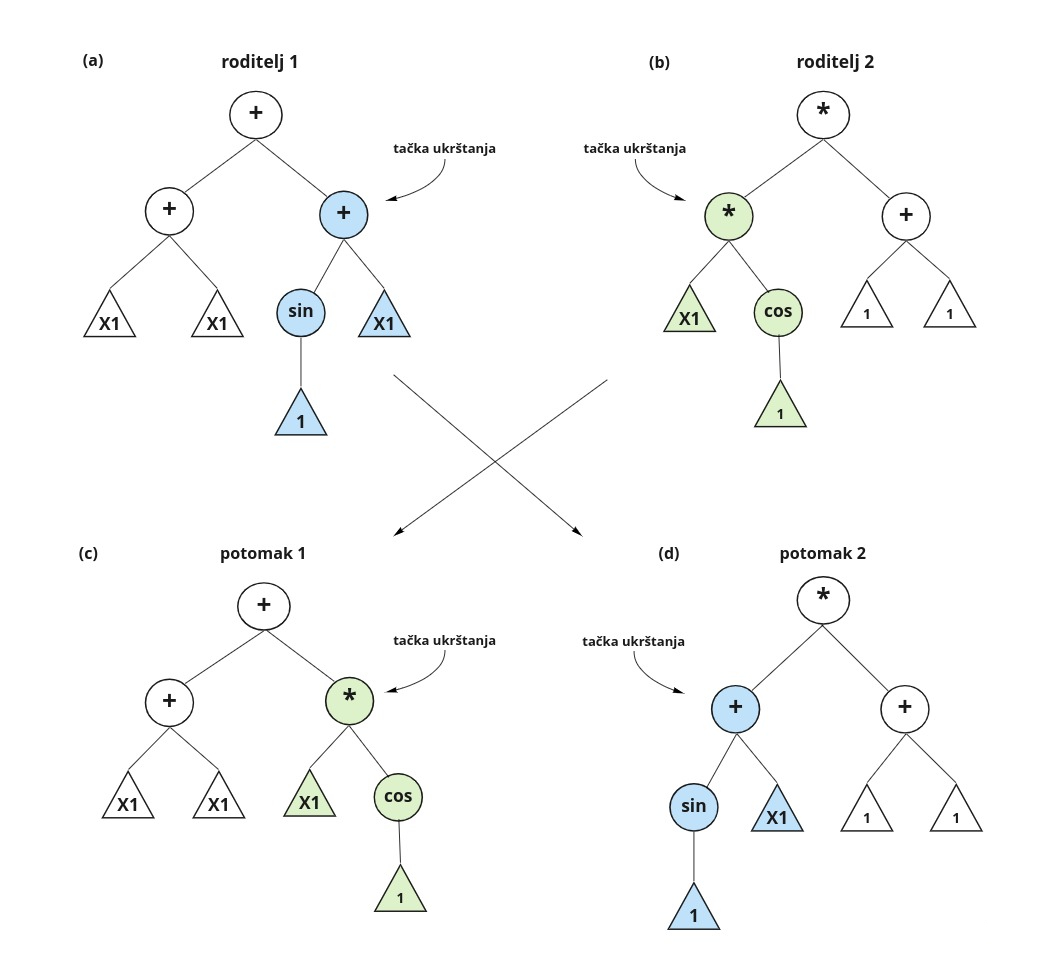
\includegraphics[width=0.65\textwidth]{images/standard_crossover4.jpg}
\end{center}
\label{fig:standardCrossover}
\end{figure}

\end{frame}


\begin{frame}{Operatori ukrštanja - Operator zasnovan na semantičkoj sličnosti}
\begin{itemize}
\small
    \item \textit{Semantika uzorkovanja} (SS) nekog podstabla se aproksimira pomoću vrednosti dobijenih evaluacijom tog podstabla na predefinisanom skupu tačaka iz domena problema.
    \item Neka je $F$ funkcija koja je izražena pomoću (pod)stabla $T$ na domenu $D$ i neka je $P$ skup tačaka iz domena $D$, $P = \{p_1, p_2, ..., p_N\}$. Tada je \textit{semantika uzorkovanja} stabla $T$ na skupu $P$ u domenu $D$, skup $S = \{s_1, s_2, ..., s_N\}$ takav da je $s_i = F(p_i), i=1,2,..,N$.
    \item \textit{Rastojanje semantike uzorkovanja} (SSD) između dva podstabla: Neka je $P = \{p_1, p_2, ..., p_N\}$ \textit{semantika uzorkovanja} podstabla $St_1$, a $Q = \{q_1, q_2, ..., q_N\}$ \textit{semantika uzorkovanja} podstabla $St_2$. Onda se $SSD$ između $St_1$ i $St_2$ definiše kao 
    \[ SSD(St_1, St_2) = \frac{1}{N}(|p_1 - q_1| + |p_2 - q_2| + ... + |p_N - q_N|). \]
\end{itemize}
\end{frame}

\iffalse
\begin{frame}{Operatori ukrštanja - Operatori zasnovani na semantici}
\begin{itemize}
    \item Pomoću $SSD$ se definišu \textit{semantička ekvivalentnost} i \textit{semantička sličnost} između dva podstabla.
    \item Dva podstabla su \textit{semantički ekvivalentna} (SE, eng. \textit{Semantically Equivalent}) na domenu ako je njihova $SSD$ vrednost dovoljno mala
    
    \[
        SE(St_1, St_2)= 
    \begin{dcases}
        true,& \text{ako je } SSD(St_1, St_2) < \epsilon\\
        false,              & \text{inače}
    \end{dcases}
    \]
    
    \item Parametar $\epsilon$ predstavlja \textit{semantičku osetljivost} (eng. \textit{semantic sensitivity}). Za njega je najbolje uzeti neku vrednost iz skupa \{0.01, 0.02, 0.04, 0.05, 0.06, 0.08, 0.1\}.

\end{itemize}
\end{frame}
\fi
    

\begin{frame}{Operatori ukrštanja - Operator zasnovan na semantičkoj sličnosti}
\begin{itemize}
\small
    %\item Pomoću $SSD$ se definiše \textit{semantička sličnost}.
    \item Dva podstabla su \textit{semantički slična} ($SS_i$) na domenu ako njihova $SSD$ vrednost leži na nekom pozitivnom intervalu.
    \scriptsize
    \[
        SS_i(St_1, St_2)= 
    \begin{dcases}
        true,& \text{ako je } \alpha < SSD(St_1, St_2) < \beta\\
        false,              & \text{inače}
    \end{dcases}
    \]
    \small
    %\item Parametri $\alpha$ i $\beta$ donja i gornja granica semantičke osetljivosti (LBSS, eng. \textit{Lower Bound Semantic Sensitivity} i UBSS, eng. \textit{Upper Bound Semantic Sensitivity}). Kod simboličke regresije najbolje rezultate daju vrednosti između 0.4 i 0.6 za $UBSS$, a vrednosti $10^{-2}$ ili manje za $LBSS$.
    %\item Motivacija za korišćenje semantičke sličnosti - verovatnije je da će razmena podstabala biti korisnija ukoliko se odvija izmed̄u dve jedinke koje nisu semantički identične, ali nisu ni semantički suviše različite.
    \item Operator ukrštanja zasnovan na semantičkoj sličnosti (SSC) -- ukrštanje samo semantički sličnih podstabala.
    %\item Semantičku sličnost mnogo teže zadovoljiti -- dolaziće do uzastopnih neuspešnih pokušaja tokom potrage za takvim podstablima.
    \item Koristi se veći broj pokušaja za pronalazak semantički sličnog para.
    \item Ako se pređe dozvoljeni broj pokušaja, podstabla se biraju na slučajan način.
\end{itemize}
\end{frame}


\iffalse
\begin{frame}{Operatori ukrštanja - Operatori zasnovani na semantici}
\small
\textbf{Operator ukrštanja koji je svestan semantike, SAC (eng. Semantics Aware Crossover)}
\begin{itemize}
    \item Onemogućavanje razmene semantički ekvivalentnih podstabala koji dovode do kreiranja potomaka koji su identični svojim roditeljima.
    
    \begin{figure}[!ht]
    \begin{center}
    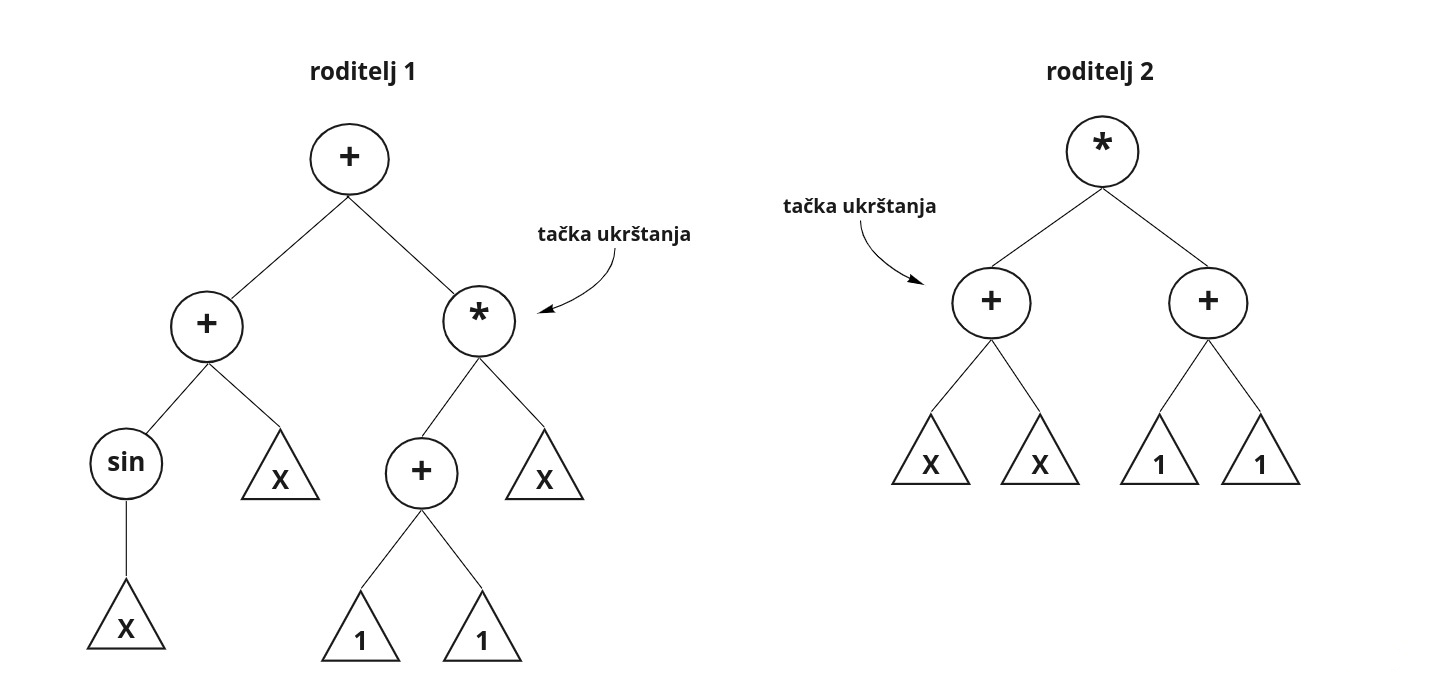
\includegraphics[width=0.6\textwidth]{images/SAC1.jpg}
    \end{center}
    \label{fig:sac1}
    \end{figure} 
    
    \item Ako su podstabla ekvivalentna, ponovo se na slučajan način biraju tačke ukrštanja.
\end{itemize}
\end{frame}
\fi



\begin{frame}{Operatori mutacije}
\begin{enumerate}

\begin{figure}[!ht]
\begin{center}
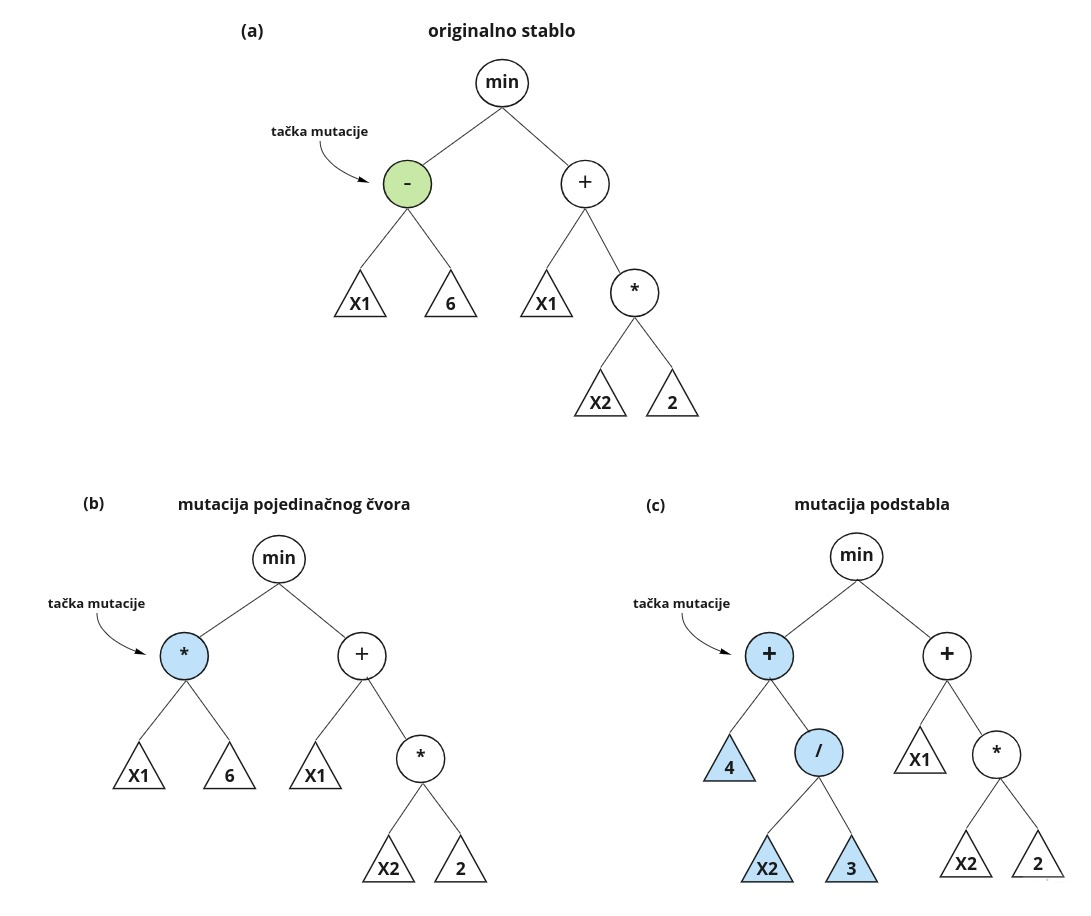
\includegraphics[width=0.65\textwidth]{images/mutation4.jpg}
\end{center}
\label{fig:mutation}
\end{figure}

\end{enumerate}
\end{frame}



\begin{frame}{Metoda promenljivih okolina}
\begin{enumerate}
  \item Inicijalizacija: Izbor skupa okolina $N_k, k = 1, ..., k_{max}$; Konstruisanje početnog rešenja x;
  \item Ponavljanje narednih koraka sve dok se ne ispuni kriterijum zaustavljanja:
  \begin{enumerate}
    \item Postaviti k = 1;
    \item Ponavljati naredne korake sve dok je $k \leq k_{max}$
        \begin{enumerate}
        \item \textit{Razmrdavanje} - Generisanje slučajnog rešenja $x_1$ iz okoline $N_k(x)$;
        \item \textit{Lokalna pretraga} - Primeniti neku metodu lokalne pretrage sa početnim rešenjem $x_1$. Rezultat pretrage označiti sa $x_2$;
        \item \textit{Prihvatanje rešenja i promena okoline} - Ako je dobijeno rešenje $x_2$ bolje od  $x$, postaviti $x$ = $x_2$ i  $k = 1$; Inače, postaviti $k = k + 1$;
      \end{enumerate}
  \end{enumerate}
\end{enumerate}
Kriterijum zaustavljanja može biti pronalazak tačnog rešenja (određen pomoću $R^2$), maksimalan dozvoljeni broj iteracija ili maksimalno vreme izvršavanja.
\end{frame}

\subsection{Metoda promenljivih okolina}
\begin{frame}{Tipovi okolina i razmrdavanje}
Tipovi okolina:
\begin{enumerate}
    \item  $N(T)$ - struktura susedstva koje se koristi tokom lokalne pretrage. Članovi ove vrste susedstva se formiraju elementarnim transformacijama stabla.
    \item $N_1(T)$ - struktura susedstva čiji se članovi dobijaju mutacijom pojedinačnog čvora.
    \item $N_2(T)$ - struktura susedstva čiji se članovi dobijaju mutacijom celog podstabla.
\end{enumerate}
Okoline $N_1(T)$ i $N_2(T)$ se koriste u proceduri razmrdavanja.

Razmrdavanje:
\begin{enumerate}
    \item Dobija se $k$-ti sused stabla $T$, primenom istog poteza $k$ puta.
    \item Prvo se nasumičnobira okolina $N_1(T)$ ili $N_2(T)$, a zatim se taj operator primenjuje $k$ puta nad datim stablom.
\end{enumerate}
\end{frame}


\begin{frame}{Elementarne transformacije stabla (ETT) i lokalna pretraga}
\begin{itemize}
\small
    \item Elementarne transformacije stabla (ETT): Neka je $G(V, E)$ neusmereni graf i neka je $T(V, A)$ neko razapinjuće stablo grafa $G$. ETT transformiše stablo $T$ u stablo $T'$ (u oznaci $T' = ETT(T)$) sledećim koracima:
    \begin{itemize}
        \item U stablo $T$ dodati granu $a$, takvu da $a \in E \setminus A$.
        \item Detektovati formirani ciklus i ukloniti bilo koju granu (osim one koja je dodata u prethodnom koraku) iz njega kako bi se dobio podgraf $T'$, koji takođe predstavlja razapinjuće stablo grafa $G$.
    \end{itemize}
    \item Strategija \textit{prvog poboljšanja}%: Kada se naiđe na prvo stablo koje daje bolje rezultate na datom skupu podataka, ono se vraća kao trenutno najbolje rešenje iz čijeg susedstva će se dalje nastaviti pretraga.
    \item Poređenje kvalieta stabala -- koeficijent determinacije $R^{2}$. 
\end{itemize}
\end{frame}


\iffalse
\begin{frame}{Elementarne transformacije stabla (ETT) i lokalna pretraga}
\small
Naredbe algoritma EET se se mogu grupisati u četiri grupe:
\begin{enumerate}
    \item \textit{Dodavanje grane (tip I)}. Grana $(i,j)$ se dodaje u trenutno stablo $T$, pri čemu ni $i$ ni $j$ ne smeju biti koren stabla. Dodatno, ili $i$ ili $j$ mora da bude funkcija. Nakon primene ovog koraka se formira ciklus u trenutnom stablu.
    \item \textit{Uklanjanje grane (tip I)}. Ovde postoje dva slučaja. Ako su i $i$ i $j$ funkcije, onda se može ukloniti neka od grana $(i, parent(i))$, $(j, parent(j))$ kako bi se uklonio ciklus. Ako je jedan od čvorova terminal, npr. neka to bude $j$, onda se uklanja grana $(j, parent(j))$.
    \item \textit{Dodavanje grane (tip II)}. Ako je obrisana grana $(i, parent(i))$, onda se dodaje grana $(parent(i), child(j))$. Ako je obrisana grana $(j, parent(j))$, onda se dodaje grana $(parent(j), child(i))$. 
    \item \textit{Uklanjanje grane (tip II)}. Uklanjaju se odgovarajuće grane kako bi stepen čvorova ostao zadovoljavajući. 
\end{enumerate}
\end{frame}
\fi


\section{Eksperimentalni rezultati}

\begin{frame}{Podaci}
Sve metode su testirane pomoću tri vrste skupova podataka:
\begin{enumerate}
\small
    \item Skup podataka generisan na osnovu funkcija koje se često razmatraju u literaturi. Za svaku funkciju je generisano 100 instanci na osnovu slučajno odabranih vrednosti nezavisnih promenljiih. 
    
    $ F_1 = x^3 + x^2 + x, \quad x \in [-1, 1] $

    $ F_2 = x^4 + x^3 + x^2 + x, \quad x \in [-1, 1] $
    
    $ F_3 = x^5 + x^4 + x^3 + x^2 + x, \quad x \in [-1, 1] $
    
    $ F_4 = x^6 + x^5 + x^4 + x^3 + x^2 + x, \quad x \in [-1, 1] $
    
    $ F_5 = sin(x^2)cos(x) - 1, \quad x \in [-1, 1] $
    
    $ F_6 = sin(x) + sin(x + x^2), \quad x \in [-1, 1] $
    
    $ F_7 = log(x + 1) + log(x^2 + 1), \quad x \in [0, 2] $
    
    $ F_8 = sin(x_0) + sin(x_1^2), \quad x_0, x_1 \in [-1, 1] $
    
    $ F_9 = 2sin(x_0)cos(x_1), \quad x_0, x_1 \in [-1, 1] $
\end{enumerate}
\end{frame}

\begin{frame}{Podaci}
\begin{enumerate}
\setcounter{enumi}{1}
    \item Skup podataka generisan na osnovu jednostavnijih funkcija radi upoređivanja metaheurističkih metoda sa metodom grube sile.
    
    $F_{01} = x_0 x_1 + x_1$

    $F_{02} = x_1 + x_1^2 + x_0$
    
    $F_{03} = x_0 x_1 + cos(x_0)$
    
    $F_{04} = x_0 - x_1 x_1$
    
    $F_{05} = x_0 - x_1 x_1 + x_1$
\end{enumerate}
\begin{enumerate}
\setcounter{enumi}{2}
    \item Jedan od javno dostupnih skupova podataka za regresiju - $"$Yacht Hydrodynamics$"$ skup. Skup sadrži 308 instanci koje su određene pomoću 6 nezavisnih i jedne ciljne promenljive. Sve vrednosti su realnog tipa.
\end{enumerate}
\end{frame}


\begin{frame}{Rezultati}
\small
Poređenje sa algoritmom grube sile:
\begin{itemize}
    \item Algoritam grube sile -- optimalno rešenje za $F_{01}, ..., F_{05}$ i $F_{1}$ i $F_{2}$. U ostalim primerima je dolazilo do nedostatka memorijskih resursa.
    \item Svi metaheuristički pristupi - optimalno rešenje za primere $F_{01},.., F_{05}$.
\end{itemize}
Poređenje metaheurističkih metoda:
\begin{itemize}
    \item Svaki skup podataka je podeljen na trening (70\%) i test (30\%) deo.
    \item Svaka metoda je evaluirana tako što je pokrenuta po 30 puta nad svim skupovima podataka -- u svakom pokretanju je dobijen najbolji izraz.
    %\item Prilikom svakog od tih nezavisnih pokretanja dobijen je izraz koji u tom izvršavanju najbolje odgovara datom skupu podataka. 
    \item Za taj izraz je izračunat $R^2$ na trening i test skupu i provereno je da li i simbolički odgovara ciljnom izrazu.
    \item Pri svakom pokretanju mereno je i vreme koje je bilo potrebno za pronalazak najboljeg rešenja.
\end{itemize}
\end{frame}


%------------------------------------------


\begin{frame}{Evaluacija i poređenje metaheurističkih metoda}
\scriptsize

\newcolumntype{?}{!{\vrule width 1pt}}
\begin{table}
\caption{Prosečne vrednosti određenih karakteristika u 30 nezavisnih pokretanja}
\begin{center}
\begin{tabular}{ |c?|c|c|c?|c|c|c?| } 
\hline
& \multicolumn{3}{|c?|}{\thead{Prosečna \bm{$R^2$} vrednost \\ na  trening skupu}} & \multicolumn{3}{|c?|}{\thead{Prosečna \bm{$R^2$} vrednost \\ na test skupu}} \\
\hline
& \textbf{GP} & \textbf{GP sa SSC} & \textbf{VNP} & \textbf{GP} & \textbf{GP sa SSC} & \textbf{VNP} \\
\hline
$\boldsymbol F_{\boldsymbol 0 \boldsymbol 1}$ & 0.879 & 0.831 & \textbf{0.949} & 0.898 & 0.861 & \textbf{0.945} \\
\hline
$\boldsymbol F_{\boldsymbol 0 \boldsymbol 2}$ & 0.765 & 0.802 & \textbf{0.848} & 0.791 & 0.818 & \textbf{0.897} \\
\hline
$\boldsymbol F_{\boldsymbol 0 \boldsymbol 3}$ & 0.745 & 0.733 & \textbf{0.863} & 0.810 & 0.820 & \textbf{0.926} \\
\hline
$\boldsymbol F_{\boldsymbol 0 \boldsymbol 4}$ & 0.733 & 0.740 & \textbf{0.914} & 0.820 & 0.775 & \textbf{0.922} \\
\hline
$\boldsymbol F_{\boldsymbol 0 \boldsymbol 5}$ & 0.795 & 0.771 & \textbf{0.846} & 0.797 & 0.765 & \textbf{0.813} \\
\hline
\end{tabular}
\end{center}
\end{table}
\end{frame}




\begin{frame}{Evaluacija i poređenje metaheurističkih metoda}
\scriptsize

\newcolumntype{?}{!{\vrule width 1pt}}
\begin{table}
\caption{Prosečne vrednosti određenih karakteristika u 30 nezavisnih pokretanja}
\begin{center}
\begin{tabular}{ |c?|c|c|c?|c|c|c?| } 
\hline
& \multicolumn{3}{|c?|}{\thead{Broj pokretanja u kojima je \\ pronađeno rešenje \\ simbolički ekvivalentno \\ ciljnom rešenju}} & \multicolumn{3}{|c|}{\thead{Prosečno vreme \\ izvršavanja (s)}}  \\
\hline
& \textbf{GP} & \textbf{GP sa SSC} & \textbf{VNP} & \textbf{GP} & \textbf{GP sa SSC} & \textbf{VNP} \\
\hline
$\boldsymbol F_{\boldsymbol 0 \boldsymbol 1}$ & 7 & 3 & \textbf{13} & 12 & 19 & \textbf{4} \\
\hline
$\boldsymbol F_{\boldsymbol 0 \boldsymbol 2}$ & 1 & 3 & \textbf{11} & 7 & 13 & \textbf{6} \\
\hline
$\boldsymbol F_{\boldsymbol 0 \boldsymbol 3}$ & 5 & 5 & \textbf{14} & 6 & 12 & \textbf{5} \\
\hline
$\boldsymbol F_{\boldsymbol 0 \boldsymbol 4}$ & 2 & 1 & \textbf{9} & 12 & 18 & \textbf{5} \\
\hline
$\boldsymbol F_{\boldsymbol 0 \boldsymbol 5}$ & 3 & 1 & \textbf{9} & \textbf{7} & 18 & \textbf{7} \\
\hline
\end{tabular}
\end{center}
\end{table}

\end{frame}


%  ////////////////////////////////




\begin{frame}{Evaluacija i poređenje metaheurističkih metoda}
\scriptsize
\newcolumntype{?}{!{\vrule width 1pt}}
\begin{table}
\caption{Prosečne vrednosti određenih karakteristika u 30 nezavisnih pokretanja}
\label{tbl:meanVals2}
\begin{center}
\begin{tabular}{ |c?|c|c|c?|c|c|c?| } 
\hline
& \multicolumn{3}{|c?|}{\thead{Prosečna \bm{$R^2$} vrednost \\ na  trening skupu}} & \multicolumn{3}{|c?|}{\thead{Prosečna \bm{$R^2$} vrednost \\ na test skupu}}  \\
\hline
& \textbf{GP} & \textbf{GP sa SSC} & \textbf{VNP} & \textbf{GP} & \textbf{GP sa SSC} & \textbf{VNP} \\
\hline
$\boldsymbol F_{\boldsymbol 1}$ & \textbf{0.914} & 0.861 & 0.907 & \textbf{0.907} & 0.827 & 0.872 \\
\hline
$\boldsymbol F_{\boldsymbol 2}$ & \textbf{0.827} & 0.799 & 0.771 & \textbf{0.824} & 0.798 & 0.770 \\
\hline
$\boldsymbol F_{\boldsymbol 3}$ & \textbf{0.851} & 0.851 & 0.797 & 0.695 & -1.428 & \textbf{0.752} \\
\hline
$\boldsymbol F_{\boldsymbol 4}$ & 0.746 & 0.691 & \textbf{0.809} & \textbf{0.796} & 0.743 & 0.778 \\
\hline
$\boldsymbol F_{\boldsymbol 5}$ & 0.643 & 0.606 & \textbf{0.894} & 0.607 & 0.589 & \textbf{0.887} \\
\hline
$\boldsymbol F_{\boldsymbol 6}$ & 0.928 & 0.917 & \textbf{0.945} & 0.883 & 0.881 & \textbf{0.930} \\
\hline
$\boldsymbol F_{\boldsymbol 7}$ & 0.960 & 0.968 & \textbf{0.994} & 0.950 & 0.959 & \textbf{0.993} \\
\hline
$\boldsymbol F_{\boldsymbol 8}$ & 0.857 & 0.837 & \textbf{0.968} & 0.716 & 0.657 & \textbf{0.936} \\
\hline
$\boldsymbol F_{\boldsymbol 9}$ & 0.950 & 0.940 & \textbf{0.963} & 0.955 & 0.938 & \textbf{0.971} \\
\hline
\textbf{Yacht} & 0.238 & 0.213 & \textbf{0.477} & 0.264 & 0.233 & \textbf{0.457} \\
\hline
\end{tabular}
\end{center}
\end{table}
\end{frame}



\begin{frame}{Evaluacija i poređenje metaheurističkih metoda}
\scriptsize
\newcolumntype{?}{!{\vrule width 1pt}}
\begin{table}
\caption{Prosečne vrednosti određenih karakteristika u 30 nezavisnih pokretanja}
\label{tbl:meanVals2}
\begin{center}
\begin{tabular}{ |c?|c|c|c?|c|c|c?| } 
\hline
& \multicolumn{3}{|c?|}{\thead{Broj pokretanja u kojima je \\ pronađeno rešenje \\ simbolički ekvivalentno \\ ciljnom rešenju}} & \multicolumn{3}{|c|}{\thead{Prosečno vreme \\ izvršavanja (s)}}  \\
\hline
& \textbf{GP} & \textbf{GP sa SSC} & \textbf{VNP} & \textbf{GP} & \textbf{GP sa SSC} & \textbf{VNP}  \\
\hline
$\boldsymbol F_{\boldsymbol 1}$ & 0 & 0 & \textbf{13} & 15 & 24 & \textbf{7} \\
\hline
$\boldsymbol F_{\boldsymbol 2}$ & 0 & 0 & \textbf{9} & 13 & 26 & \textbf{9} \\
\hline
$\boldsymbol F_{\boldsymbol 3}$ & 0 & 0 & \textbf{2} & 20 & 23 & \textbf{10} \\
\hline
$\boldsymbol F_{\boldsymbol 4}$ & 0 & 0 & \textbf{2} & 14 & 27 & \textbf{12} \\
\hline
$\boldsymbol F_{\boldsymbol 5}$ & 0 & 0 & 0 & \textbf{14} & 24 & \textbf{14} \\
\hline
$\boldsymbol F_{\boldsymbol 6}$ & 0 & 0 & \textbf{1} & 13 & 27 & \textbf{12} \\
\hline
$\boldsymbol F_{\boldsymbol 7}$ & 0 & 0 & 0 & 18 & 51 & \textbf{13} \\
\hline
$\boldsymbol F_{\boldsymbol 8}$ & 0 & 0 & \textbf{3} & 13 & 35 & \textbf{7} \\
\hline
$\boldsymbol F_{\boldsymbol 9}$ & 1 & 1 & \textbf{2} & 12 & 28 & \textbf{8} \\
\hline
\textbf{Yacht} & / & / & / & 183 & 247 & \textbf{30} \\
\hline
\end{tabular}
\end{center}
\end{table}
\end{frame}



%///////////////////////////////////////



%-------------------------------------------------------------------------



\begin{frame}{Evaluacija i poređenje metaheurističkih metoda}
\tiny
\newcolumntype{?}{!{\vrule width 1pt}}
\begin{table}
\caption{Informacije o izrazu koji daje maksimalnu $R^2$ vrednost na test skupu od svih izraza dobijenih pri 30 nezavisnih pokretanja}
\label{tbl:maxVals1}
\begin{center}
\begin{tabular}{ |c?|c|c|c?|c|c|c?| } 
\hline
& \multicolumn{3}{|c?|}{\thead{Maksimalna \bm{$R^2$} vrednost \\ na  test skupu}} & \multicolumn{3}{|c?|}{\thead{Izraz koji ima maksimalnu \\ \bm{$R^2$} vrednost na test skupu}} \\
\hline
& \textbf{GP} & \textbf{GP sa SSC} & \textbf{VNP} & \textbf{GP} & \textbf{GP sa SSC} & \textbf{VNP} \\
\hline
$\boldsymbol F_{\boldsymbol 0 \boldsymbol 1}$ & 1.0 & 1.0 & 1.0 & $x_1(x_0$ + $1)$ & $x_1(x_0$ + $1)$ & $x_1(x_0$ + $1)$ \\
\hline
$\boldsymbol F_{\boldsymbol 0 \boldsymbol 2}$ & 1.0 & 1.0 & 1.0 & $x_0$ + $x_1^2$ + $x_1$ & $x_0$ + $x_1^2$ + $x_1$ & $x_0$ + $x_1^2$ + $x_1$  \\
\hline
$\boldsymbol F_{\boldsymbol 0 \boldsymbol 3}$ & 1.0 & 1.0 & 1.0 & $x_0 x_1$ + $cos(x_0)$ & $x_0 x_1$ + $cos(x_0)$ & $x_0 x_1$ + $cos(x_0)$ \\
\hline
$\boldsymbol F_{\boldsymbol 0 \boldsymbol 4}$ & 1.0 & 1.0 & 1.0 & $x_0 - x_1^2$ & $x_0 - x_1^2$ & $x_0 - x_1^2$  \\
\hline
$\boldsymbol F_{\boldsymbol 0 \boldsymbol 5}$ & 1.0 & 1.0 & 1.0 & $x_0 - x_1^2$ + $x_1$ & $x_0 - x_1^2$ + $x_1$ & $x_0 - x_1^2$ + $x_1$ \\
\hline
\end{tabular}
\end{center}
\end{table}

\begin{itemize}
\normalsize
    \item Sve metode su pronašle izraze koji su ekvivalentni sa ciljnim izrazom.
    \item Za istu instancu, sve metode su vratile isti izraz.
\end{itemize}


\end{frame}


\iffalse
\begin{frame}{Evaluacija i poređenje metaheurističkih metoda}
\scriptsize
\newcolumntype{?}{!{\vrule width 1pt}}
\begin{table}
\caption{Informacije o izrazu koji daje maksimalnu $R^2$ vrednost na test skupu od svih izraza dobijenih pri 30 nezavisnih pokretanja}
\label{tbl:maxVals1}
\begin{center}
\begin{tabular}{ |c?|c|c|c?| } 
\hline
& \multicolumn{3}{|c|}{\thead{Simbolička \\ ekvivalencija sa \\ ciljnim izrazom}} \\
\hline
& \textbf{GP} & \textbf{GP sa SSC} & \textbf{VNP} \\
\hline
$\boldsymbol F_{\boldsymbol 0 \boldsymbol 1}$ & Da & Da & Da \\
\hline
$\boldsymbol F_{\boldsymbol 0 \boldsymbol 2}$ & Da & Da & Da \\
\hline
$\boldsymbol F_{\boldsymbol 0 \boldsymbol 3}$ & Da & Da & Da \\
\hline
$\boldsymbol F_{\boldsymbol 0 \boldsymbol 4}$ & Da & Da & Da \\
\hline
$\boldsymbol F_{\boldsymbol 0 \boldsymbol 5}$ & Da & Da & Da \\
\hline
\end{tabular}
\end{center}
\end{table}
\end{frame}
\fi

%///////////////////////////////////////
% -------------------


\begin{frame}{Evaluacija i poređenje metaheurističkih metoda}
\tiny
\newcolumntype{?}{!{\vrule width 1pt}}
\renewcommand{\arraystretch}{1.0}
\begin{table}
\caption{Informacije o izrazu koji daje maksimalnu $R^2$ vrednost na test skupu od svih izraza dobijenih pri 30 nezavisnih pokretanja}
\label{tbl:maxVals2}
\begin{center}
\begin{tabular}{ |c?|c|c|c?|c|c|c| } 
\hline
& \multicolumn{3}{|c?|}{\thead{Maksimalna \\ \bm{$R^2$} vrednost \\ na  test skupu}} & \multicolumn{3}{|c|}{\thead{Simbolička \\ ekvivalencija sa \\ ciljnim izrazom}} \\
\hline
& \textbf{GP} & \textbf{\thead{GP \\ sa SSC}} & \textbf{VNP} & \textbf{GP} & \textbf{\thead{GP \\ sa SSC}} & \textbf{VNP} \\
\hline
$\boldsymbol F_{\boldsymbol 1}$ & 0.992 & 0.985 & \textbf{1.0} & Ne & Ne & \textbf{Da} \\
\hline
$\boldsymbol F_{\boldsymbol 2}$ & 0.994 & 0.981 & \textbf{1.0} & Ne & Ne & \textbf{Da} \\
\hline
$\boldsymbol F_{\boldsymbol 3}$ & 0.981 & 0.995 & \textbf{1.0} & Ne & Ne & \textbf{Da} \\
\hline
$\boldsymbol F_{\boldsymbol 4}$ & 0.986 & 0.960 & \textbf{1.0} & Ne & Ne & \textbf{Da}  \\
\hline
$\boldsymbol F_{\boldsymbol 5}$ & 0.943 & 0.964 & \textbf{0.999} & Ne & Ne & Ne \\
\hline
$\boldsymbol F_{\boldsymbol 6}$ & 0.971 & 0.987 & \textbf{1.0} & Ne & Ne & \textbf{Da} \\
\hline
$\boldsymbol F_{\boldsymbol 7}$ & 0.997 & 0.998 & \textbf{0.999} & Ne & Ne & Ne \\
\hline
$\boldsymbol F_{\boldsymbol 8}$ & 0.999 & 0.994 & \textbf{1.0} & Ne & Ne & \textbf{Da} \\
\hline
$\boldsymbol F_{\boldsymbol 9}$ & \textbf{1.0} & \textbf{1.0} & \textbf{1.0} & \textbf{Da} & \textbf{Da} & \textbf{Da} \\
\hline
\textbf{Yacht} & 0.929 & 0.792 & \textbf{0.956} & / & / & / \\
\hline 
\end{tabular}
\end{center}
\end{table}

\end{frame}

\iffalse
\begin{frame}{Evaluacija i poređenje metaheurističkih metoda}
\scriptsize
\begin{table}
\def\arraystretch{1.5}
\caption{Informacije o izrazu koji daje maksimalnu $R^2$ vrednost na test skupu od svih izraza dobijenih pri 30 nezavisnih pokretanja za ''Yacht Hydrodynamics'' skup podataka}
\label{tbl:maxVals3}
\begin{center}
\setlength{\extrarowheight}{4pt}
\begin{tabular}{ |c|c|c|c|c| } 
\hline
\thead{Metoda} & \thead{Maksimalna \bm{$R^2$} \\ vrednost na \\ test skupu} & \thead{Izraz koji ima \\ maksimalnu \bm{$R^2$} \\ vrednost na \\ test skupu } \\
\hline
{GP} & 0.929 & $1.906^{(3.963 x_5)}$  \\
\hline
{GP sa SSC} & 0.792 & $ \frac{0.822}{0.052^{x_5}} $ \\
\hline
{VNP} 
& \textbf{0.956} & $ 0.000196^{\frac{x_1 - x_2 x_5}{x_2}  * \frac{x_5}{x_1 - 2 x_5^2} } $ \\
\hline
\end{tabular}
\end{center}
\end{table}
\end{frame}
\fi

\iffalse
\section{Literatura}
\begin{frame}[allowframebreaks]
        \frametitle{Literatura}
        \bibliographystyle{abbrv}
        \bibliography{literature.bib}
\end{frame}
\fi

\setbeamertemplate{footline}{\hspace*{.5cm}\scriptsize{\hspace*{50pt} \hfill\hspace*{.5cm} \setbeamercolor{black}}\\
\vspace{9pt}}

\setbeamertemplate{headline}{\hspace*{.5cm}\scriptsize{\hspace*{50pt} \hfill\hspace*{.5cm} \setbeamercolor{black}}\\
\vspace{1pt}}

% \setbeamercolor{mysection in head/foot}{bg= black,fg=black}
\end{document}